\documentclass[11pt]{article}
\usepackage{amsmath}
\usepackage{amssymb}
\usepackage{graphicx}
\usepackage{tabularx}
\usepackage{fancyhdr}
\usepackage{lastpage}

% Page layout
\usepackage[top=1in, bottom=1in, left=1in, right=1in]{geometry}

% Header and footer
\pagestyle{fancy}
\fancyhf{}
\rfoot{Page \thepage}
\renewcommand{\headrulewidth}{0pt}

% Modified Question command with left-aligned number
\newcommand{\questiona}[2]{
    \noindent\textbf{Q#2.} #1 \hfill \textbf{[1 Mark]}
}

\newcommand{\questionb}[2]{
    \noindent\textbf{Q#2.} #1 \hfill \textbf{[2 Marks]}
}

\begin{document}

% Title section with horizontal line
\begin{center}
    \Large\textbf{GATE 2018 - Textile Engineering and Fibre Science (TF)} \\
    \large\textbf{General Aptitude and Technical Questions} \\
    \rule{\textwidth}{0.5pt} % Horizontal line below heading
\end{center}

\vspace{0.5cm}

% General Aptitude Section
\section*{General Aptitude}

\questiona{“When she fell down the \_\_\_\_\_, she received many \_\_\_\_\_ but little help.”}{1}
\begin{enumerate}
    \item[(A)] stairs, stares
    \item[(B)] stairs, stairs
    \item[(C)] stares, stairs
    \item[(D)] stares, stares
\end{enumerate}
\vspace{0.5cm}

\questiona{In spite of being warned repeatedly, he failed to correct his \_\_\_\_\_ behaviour.}{2}
\begin{enumerate}
    \item[(A)] rational
    \item[(B)] reasonable
    \item[(C)] errant
    \item[(D)] good
\end{enumerate}
\vspace{0.5cm}

\questiona{For \(0 \leq x \leq 2\pi\), \(\sin x\) and \(\cos x\) are both decreasing functions in the interval \_\_\_\_\_.}{3}
\begin{enumerate}
    \item[(A)] \( (0, \frac{\pi}{2}) \)
    \item[(B)] \( (\frac{\pi}{2}, \pi) \)
    \item[(C)] \( (\pi, \frac{3\pi}{2}) \)
    \item[(D)] \( (\frac{3\pi}{2}, 2\pi) \)
\end{enumerate}
\vspace{0.5cm}

\questiona{The area of an equilateral triangle is \(\sqrt{3}\). What is the perimeter of the triangle?}{4}
\begin{enumerate}
    \item[(A)] 2
    \item[(B)] 4
    \item[(C)] 6
    \item[(D)] 8
\end{enumerate}
\vspace{0.5cm}

\questiona{Arrange the following three-dimensional objects in the descending order of their volumes: \\
(i) A cuboid with dimensions 10 cm, 8 cm and 6 cm \\
(ii) A cube of side 8 cm \\
(iii) A cylinder with base radius 7 cm and height 7 cm \\
(iv) A sphere of radius 7 cm}{5}
\begin{enumerate}
    \item[(A)] (i), (ii), (iii), (iv)
    \item[(B)] (ii), (i), (iv), (iii)
    \item[(C)] (iii), (ii), (i), (iv)
    \item[(D)] (iv), (iii), (ii), (i)
\end{enumerate}
\vspace{0.5cm}

\questionb{An automobile travels from city A to city B and returns to city A by the same route. The speed of the vehicle during the onward and return journeys were constant at 60 km/h and 90 km/h, respectively. What is the average speed in km/h for the entire journey?}{6}
\begin{enumerate}
    \item[(A)] 72
    \item[(B)] 73
    \item[(C)] 74
    \item[(D)] 75
\end{enumerate}
\vspace{0.5cm}

\questionb{A set of 4 parallel lines intersect with another set of 5 parallel lines. How many parallelograms are formed?}{7}
\begin{enumerate}
    \item[(A)] 20
    \item[(B)] 48
    \item[(C)] 60
    \item[(D)] 72
\end{enumerate}
\vspace{0.5cm}

\questionb{To pass a test, a candidate needs to answer at least 2 out of 3 questions correctly. A total of 6,30,000 candidates appeared for the test. Question A was correctly answered by 3,30,000 candidates. Question B by 2,50,000 candidates. Question C by 2,60,000 candidates. Both A and B by 1,00,000 candidates. Both B and C by 90,000 candidates. Both A and C by 80,000 candidates. If the number of students answering all questions correctly is the same as the number answering none, how many candidates failed to clear the test?}{8}
\begin{enumerate}
    \item[(A)] 30,000
    \item[(B)] 2,70,000
    \item[(C)] 3,90,000
    \item[(D)] 4,20,000
\end{enumerate}
\vspace{0.5cm}

\questionb{If \(x^2 + x - 1 = 0\), what is the value of \(x^4 + \frac{1}{x^4}\)?}{9}
\begin{enumerate}
    \item[(A)] 1
    \item[(B)] 5
    \item[(C)] 7
    \item[(D)] 9
\end{enumerate}
\vspace{0.5cm}

\questionb{In a detailed study of annual crow births in India, it was found that there was relatively no growth during the period 2002 to 2004 and a sudden spike from 2004 to 2005. In another unrelated study, it was found that the revenue from cracker sales in India which remained fairly flat from 2002 to 2004, saw a sudden spike in 2005 before declining again in 2006. The solid line in the graph below refers to annual sale of crackers and the dashed line refers to the annual crow births in India. Choose the most appropriate inference from the above data.}{10}
\begin{center}
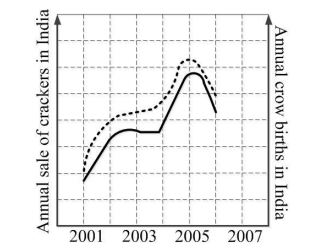
\includegraphics[width=0.5\textwidth]{figures/10.png}
\end{center}
\begin{enumerate}
    \item[(A)] There is a strong correlation between crow birth and cracker sales.
    \item[(B)] Cracker usage increases crow birth rate.
    \item[(C)] If cracker sale declines, crow birth will decline.
    \item[(D)] Increased birth rate of crows will cause an increase in the sale of crackers.
\end{enumerate}
\vspace{0.5cm}

\section*{Technical Section}

\questiona{Let \( A = \begin{bmatrix} a & b \\ 2 & -b \end{bmatrix} \) and \( X = \begin{pmatrix} -1 \\ 1 \end{pmatrix} \). If \( AX = \begin{pmatrix} -3 \\ 1 \end{pmatrix} \), then \( |A| \) is equal to}{1}
\begin{enumerate}
    \item[(A)] 2
    \item[(B)] -2
    \item[(C)] -6
    \item[(D)] 6
\end{enumerate}
\vspace{0.5cm}

\questiona{If \( A \) and \( B \) are two independent events such that \( P(A) = \frac{1}{4} \) and \( P(B) = \frac{2}{3} \), then \( P(A \cup B) \) is equal to}{2}
\begin{enumerate}
    \item[(A)] \( \frac{11}{12} \)
    \item[(B)] \( \frac{1}{12} \)
    \item[(C)] \( \frac{3}{4} \)
    \item[(D)] \( \frac{5}{6} \)
\end{enumerate}
\vspace{0.5cm}

\questiona{Which one of the following is a leaf fibre?}{3}
\begin{enumerate}
    \item[(A)] Coir
    \item[(B)] Sisal
    \item[(C)] Jute
    \item[(D)] Hemp
\end{enumerate}
\vspace{0.5cm}

\questiona{The pair of fibres most prone to accumulation of static charge is}{4}
\begin{enumerate}
    \item[(A)] Cotton and Polyester
    \item[(B)] Silk and Polyester
    \item[(C)] Polyester and Polypropylene
    \item[(D)] Silk and Polypropylene
\end{enumerate}
\vspace{0.5cm}

\questiona{Heat-setting of melt-spun and drawn Nylon 6 filament yarn under slack condition leads to increase in its}{5}
\begin{enumerate}
    \item[(A)] Tenacity
    \item[(B)] Molecular orientation
    \item[(C)] Molecular weight
    \item[(D)] Dimensional stability
\end{enumerate}
\vspace{0.5cm}

\questiona{Which one of the fibres, having stress-strain curves as shown in the figure, is the most suitable for making mountaineering ropes?}{6}
\begin{center}
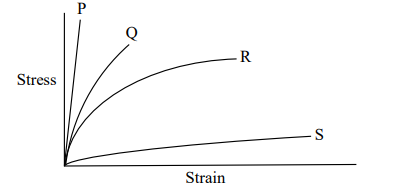
\includegraphics[width=0.5\textwidth]{figures/6.png}
\end{center}
\begin{enumerate}
    \item[(A)] P
    \item[(B)] Q
    \item[(C)] R
    \item[(D)] S
\end{enumerate}
\vspace{0.5cm}

\questiona{The technology that produces yarn with the maximum fibre migration is}{7}
\begin{enumerate}
    \item[(A)] Rotor spinning
    \item[(B)] Friction spinning
    \item[(C)] Air-jet spinning
    \item[(D)] Ring spinning
\end{enumerate}
\vspace{0.5cm}

\questiona{The cleaning machine, located in the fine cleaning zone of blowroom, uses the following as the opening element}{8}
\begin{enumerate}
    \item[(A)] Roller with saw tooth wire points
    \item[(B)] Drum with large spikes
    \item[(C)] Roller with discs having double edged teeth
    \item[(D)] Drum with large bladed discs
\end{enumerate}
\vspace{0.5cm}

\questiona{The purpose of having grooves or notches in modern flyer tops in speed frames is to}{9}
\begin{enumerate}
    \item[(A)] Increase real twist in roving
    \item[(B)] Insert false twist in roving
    \item[(C)] Reduce neps in roving
    \item[(D)] Increase fineness of roving
\end{enumerate}
\vspace{0.5cm}

\questiona{With time, wind per double traverse in a drum-driven winder}{10}
\begin{enumerate}
    \item[(A)] Increases
    \item[(B)] Decreases
    \item[(C)] Remains constant
    \item[(D)] First increases and then decreases
\end{enumerate}
\vspace{0.5cm}

\questiona{In a loom, seven-wheel take-up motion is}{11}
\begin{enumerate}
    \item[(A)] Negative and intermittent
    \item[(B)] Negative and continuous
    \item[(C)] Positive and intermittent
    \item[(D)] Positive and continuous
\end{enumerate}
\vspace{0.5cm}

\questiona{The relative humidity (in \%) and temperature (in \(^{\circ}\)C) of standard testing atmosphere are respectively}{12}
\begin{enumerate}
    \item[(A)] 65 and 25
    \item[(B)] 65 and 20
    \item[(C)] 60 and 25
    \item[(D)] 60 and 20
\end{enumerate}
\vspace{0.5cm}

\questiona{In Stelometer, if \(F\) is the force acting on a fibre bundle and \(\theta\) is the angle through which the pendulum is moved, then \(F\) is directly proportional to}{13}
\begin{enumerate}
    \item[(A)] \(\sin \theta\)
    \item[(B)] \(\cos \theta\)
    \item[(C)] \(\tan \theta\)
    \item[(D)] \(\cot \theta\)
\end{enumerate}
\vspace{0.5cm}

\questiona{Yarn diameter varies}{14}
\begin{enumerate}
    \item[(A)] Directly with yarn packing density
    \item[(B)] Inversely with yarn packing density
    \item[(C)] Directly with square root of yarn packing density
    \item[(D)] Inversely with square root of yarn packing density
\end{enumerate}
\vspace{0.5cm}

\questiona{The constant-rate-of-extension type tensile tester is NOT used for}{15}
\begin{enumerate}
    \item[(A)] Tongue tear test
    \item[(B)] Wing rip tear test
    \item[(C)] Elmendorf tear test
    \item[(D)] Trapezoid tear test
\end{enumerate}
\vspace{0.5cm}

\questiona{During bleaching of cotton with hydrogen peroxide, addition of sodium silicate}{16}
\begin{enumerate}
    \item[(A)] Reduces the viscosity of bath
    \item[(B)] Controls the rate of decomposition of perhydroxyl ions (HO\(_2^-\))
    \item[(C)] Reduces the surface tension of bath
    \item[(D)] Enhances swelling of cotton
\end{enumerate}
\vspace{0.5cm}

\questiona{In dyeing of wool with levelling acid dyes, with time, the pH of dye bath}{17}
\begin{enumerate}
    \item[(A)] Increases
    \item[(B)] Decreases
    \item[(C)] Remains constant
    \item[(D)] First increases and then decreases
\end{enumerate}
\vspace{0.5cm}

\questiona{The discharging agent used in discharge printing of cotton with reactive dyes is}{18}
\begin{enumerate}
    \item[(A)] Citric acid
    \item[(B)] Sodium dithionite
    \item[(C)] Thio-urea dioxide
    \item[(D)] Sodium formaldehyde sulphoxylate
\end{enumerate}
\vspace{0.5cm}

\questiona{Application of a fluorochemical based finish on a textile fabric imparts \\
P. Water repellency \\
Q. Oil repellency \\
R. Soil repellency \\
S. Soil release property}{19}
\begin{enumerate}
    \item[(A)] P, Q \& R only
    \item[(B)] Q, R \& S only
    \item[(C)] P, R \& S only
    \item[(D)] P, Q \& S only
\end{enumerate}
\vspace{0.5cm}

\questiona{If \( \vec{a} = -\hat{i} + 2\hat{j} \), \( \vec{b} = -\hat{j} + 2\hat{k} \) and \( \vec{c} = 2\hat{i} - \hat{k} \) are three vectors such that \( \vec{a} + \lambda \vec{b} \) is perpendicular to \( \vec{c} \), then the value of \( \lambda \) is \_\_\_\_\_\_\_\_\_\_}{20}
\vspace{0.5cm}

\questiona{If \( y(x) \) is the solution of the differential equation \( y y' = 8x \), \( y(0) = 2 \), then the absolute value of \( y(2) \) is \_\_\_\_\_\_\_\_\_\_}{21}
\vspace{0.5cm}

\questiona{If \( f(x) = \begin{cases} 4 - x, & x \leq 2 \\ kx - 4, & x > 2 \end{cases} \) is a continuous function for all real values of \( x \), then \( f(8) \) is equal to \_\_\_\_\_\_\_\_\_\_}{22}
\vspace{0.5cm}

\questiona{A twistless polyester yarn has 90 filaments, each of 2 denier. The metric count of the yarn is \_\_\_\_\_\_\_\_\_\_}{23}
\vspace{0.5cm}

\questiona{Bottom shaft of a shuttle loom, weaving 2 up 1 down twill weave, is rotating at 90 rpm. The speed of cam shaft (in rpm) is \_\_\_\_\_\_\_\_\_\_}{24}
\vspace{0.5cm}

\questiona{If wale constant and course constant for knitted fabrics are 4.2 and 5.46, respectively, then the value of the loop shape factor, accurate to one decimal place, is \_\_\_\_\_\_\_\_\_\_}{25}
\vspace{0.5cm}

\questionb{The cross-sectional shape of a fibre affects the following properties of yarn \\
P. Lustre \\
Q. Torsional rigidity \\
R. Flexural rigidity \\
S. Packing density}{26}
\begin{enumerate}
    \item[(A)] P \& Q only
    \item[(B)] P \& R only
    \item[(C)] P, Q \& R only
    \item[(D)] P, Q, R \& S
\end{enumerate}
\vspace{0.5cm}

\questionb{Determine the correctness or otherwise of the following Assertion a and the Reason r. \\
a: The reaction temperature and rate of agitation during polymerization of polyethylene terephthalate have an important effect on molecular weight of the polymer produced. \\
r: Polymerization of polyester by melt polycondensation is a predominantly diffusion controlled process.}{27}
\begin{enumerate}
    \item[(A)] Both [a] and [r] are true and [r] is the correct reason for [a]
    \item[(B)] Both [a] and [r] are true but [r] is not the correct reason for [a]
    \item[(C)] Both [a] and [r] are false
    \item[(D)] [a] is true but [r] is false
\end{enumerate}
\vspace{0.5cm}

\questionb{Group I gives a list of fibres and Group II contains their applications. Match the fibre with its application. \\
Group I \\
P. Polypropylene \\
Q. Carbon \\
R. Ultra-high molecular weight polyethylene \\
S. Meta-aramid \\
Group II \\
1. Fire proof jacket \\
2. Bullet proof jacket \\
3. Carpet \\
4. Windmill blade}{28}
\begin{enumerate}
    \item[(A)] P-4, Q-2, R-3, S-1
    \item[(B)] P-3, Q-4, R-2, S-1
    \item[(C)] P-3, Q-4, R-1, S-2
    \item[(D)] P-4, Q-1, R-2, S-3
\end{enumerate}
\vspace{0.5cm}

\questionb{Techniques used to determine the glass transition temperature of textile fibres are \\
P. X-ray diffraction (XRD) \\
Q. Differential scanning calorimetry (DSC) \\
R. Thermogravimetric analysis (TGA) \\
S. Dynamic mechanical analysis (DMA)}{29}
\begin{enumerate}
    \item[(A)] P \& Q only
    \item[(B)] Q \& R only
    \item[(C)] Q \& S only
    \item[(D)] R \& S only
\end{enumerate}
\vspace{0.5cm}

\questionb{Determine the correctness or otherwise of the following Assertion a and the Reason r. \\
a: In a carding machine, carding type of wire point configuration is used between cylinder and doffer. \\
r: Carding type of wire point configuration gives the best fibre transfer without disturbing the fibre alignment.}{30}
\begin{enumerate}
    \item[(A)] Both [a] and [r] are true and [r] is the correct reason for [a]
    \item[(B)] Both [a] and [r] are true but [r] is not the correct reason for [a]
    \item[(C)] Both [a] and [r] are false
    \item[(D)] [a] is true but [r] is false
\end{enumerate}
\vspace{0.5cm}

\questionb{Match the spinning technology listed in Group I with the machine component / function listed in Group II. \\
Group I \\
P. Wrap spinning \\
Q. Rotor spinning \\
R. Air-jet spinning \\
S. DREF II friction spinning \\
Group II \\
1. False twisting \\
2. Perforated drums \\
3. Back doubling \\
4. Hollow spindle}{31}
\begin{enumerate}
    \item[(A)] P-3, Q-4, R-2, S-1
    \item[(B)] P-4, Q-1, R-3, S-2
    \item[(C)] P-4, Q-3, R-1, S-2
    \item[(D)] P-3, Q-1, R-2, S-4
\end{enumerate}
\vspace{0.5cm}

\questionb{Compared to filaments in spunbonded nonwovens, those in meltblown nonwovens have \\
P. Lower orientation of molecular chains \\
Q. Higher orientation of molecular chains \\
R. Lower variability in diameter \\
S. Higher variability in diameter}{32}
\begin{enumerate}
    \item[(A)] P \& R only
    \item[(B)] P \& S only
    \item[(C)] Q \& R only
    \item[(D)] Q \& S only
\end{enumerate}
\vspace{0.5cm}

\questionb{Match the weave in Group I with fabric attribute in Group II. \\
Group I \\
P. Plain \\
Q. 2 up 1 down twill \\
R. 7 end satin \\
S. Mock leno \\
Group II \\
1. Holes in fabric \\
2. High tear resistance \\
3. High shear resistance \\
4. Continuous diagonal line}{33}
\begin{enumerate}
    \item[(A)] P-3, Q-4, R-2, S-1
    \item[(B)] P-1, Q-4, R-2, S-3
    \item[(C)] P-3, Q-4, R-1, S-2
    \item[(D)] P-3, Q-1, R-2, S-4
\end{enumerate}
\vspace{0.5cm}

\questionb{Match the test in Group I with fabric property in Group II. \\
Group I \\
P. Cup test \\
Q. Heart loop test \\
R. Spray rating test \\
S. Hydrostatic head test \\
Group II \\
1. Flexural rigidity \\
2. Water vapour permeability \\
3. Resistance to water penetration \\
4. Resistance to surface wettability}{34}
\begin{enumerate}
    \item[(A)] P-1, Q-2, R-3, S-4
    \item[(B)] P-1, Q-2, R-4, S-3
    \item[(C)] P-2, Q-1, R-3, S-4
    \item[(D)] P-2, Q-1, R-4, S-3
\end{enumerate}
\vspace{0.5cm}

\questionb{Determine the correctness or otherwise of the following Assertion a and the Reason r. \\
a: The work factor of silk fibre is greater than 0.5. \\
r: The work factor is calculated by assuming the following as the stress-strain curve of silk fibre.}{35}
\begin{center}
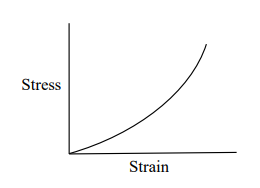
\includegraphics[width=0.5\textwidth]{figures/35.png}
\end{center}
\begin{enumerate}
    \item[(A)] Both [a] and [r] are true and [r] is the correct reason for [a]
    \item[(B)] Both [a] and [r] are true but [r] is not the correct reason for [a]
    \item[(C)] Both [a] and [r] are false
    \item[(D)] [a] is true but [r] is false
\end{enumerate}
\vspace{0.5cm}

\questionb{Determine the correctness or otherwise of the following Assertion a and the Reason r. \\
a: As the concentration of a surfactant in water increases, the surface tension of water initially decreases and then becomes constant. \\
r: After reaching the Critical Micelle Concentration, additional surfactant molecules do not further reduce the surface tension.}{36}
\begin{enumerate}
    \item[(A)] Both [a] and [r] are true and [r] is the correct reason for [a]
    \item[(B)] Both [a] and [r] are true but [r] is not the correct reason for [a]
    \item[(C)] Both [a] and [r] are false
    \item[(D)] [a] is true but [r] is false
\end{enumerate}
\vspace{0.5cm}

\questionb{A dye is applied on a fibre using Na\(_2\)S\(_2\)O\(_4\) as an auxiliary. Washing fastness of the dye on fibre is good. The correct combination of the dye and the fibre is}{37}
\begin{enumerate}
    \item[(A)] Cationic dye, acrylic fibre
    \item[(B)] Vat dye, cotton fibre
    \item[(C)] Acid dye, wool fibre
    \item[(D)] Reactive dye, cotton fibre
\end{enumerate}
\vspace{0.5cm}

\questionb{Determine the correctness or otherwise of the following Assertion a and the Reason r. \\
a: Emulsion thickener is used in pigment printing of textiles. \\
r: Emulsion thickener has high solid content.}{38}
\begin{enumerate}
    \item[(A)] Both [a] and [r] are true and [r] is the correct reason for [a]
    \item[(B)] Both [a] and [r] are true but [r] is not the correct reason for [a]
    \item[(C)] Both [a] and [r] are false
    \item[(D)] [a] is true but [r] is false
\end{enumerate}
\vspace{0.5cm}

\questionb{Match the dye-fibre in Group I with the interactions in Group II. \\
Group I \\
P. Reactive dye on cotton \\
Q. Disperse dye on polyester \\
R. Vat dye on cotton \\
S. Basic dye on acrylic \\
Group II \\
1. Van der Waals forces \\
2. Covalent bonds \\
3. Electrostatic bonds \\
4. Mechanical entrapment}{39}
\begin{enumerate}
    \item[(A)] P-1, Q-2, R-4, S-3
    \item[(B)] P-1, Q-2, R-3, S-4
    \item[(C)] P-2, Q-1, R-4, S-3
    \item[(D)] P-2, Q-1, R-3, S-4
\end{enumerate}
\vspace{0.5cm}

\questionb{Let \( X \) be a random variable following the binomial distribution. If \( E(X) = 2 \) and \( \text{Var}(X) = 1.2 \), then \( P(X = 2) \), accurate to three decimal places, is equal to \_\_\_\_\_\_\_\_\_\_}{40}
\vspace{0.5cm}

\questionb{The value of the integral \( \int_{0}^{4} \int_{0}^{\sqrt{16 - x^2}} y \sqrt{x^2 + y^2} \, dy \, dx \) is \_\_\_\_\_\_\_\_\_\_}{41}
\vspace{0.5cm}

\questionb{Starting from the initial point \( x_0 = 10 \), if the sequence \(\{x_n\}\) is generated using Newton-Raphson method to compute the root of the equation \( x^4 - 600 = 0 \), then \( x_2 \), accurate to two decimal places, is equal to \_\_\_\_\_\_\_\_\_\_}{42}
\vspace{0.5cm}

\questionb{If \( A = \begin{bmatrix} 3 & 1 \\ 1 & 3 \end{bmatrix} \), then the sum of all eigenvalues of the matrix \( M = A^2 - 4A^{-1} \) is equal to \_\_\_\_\_\_\_\_\_\_}{43}
\vspace{0.5cm}

\questionb{If the density of 100\% crystalline polyethylene is 1000 kg/m\(^3\) and that of 100\% amorphous polyethylene is 865 kg/m\(^3\), then the mass fractional crystallinity of a polyethylene fibre with density 970 kg/m\(^3\), accurate to two decimal places, is \_\_\_\_\_\_\_\_\_\_}{44}
\vspace{0.5cm}

\questionb{In winding zone of ring spinning, the permissible minimum angle of lead is \(30^\circ\). For a ring of 40 mm diameter, the minimum diameter (in mm) of bobbin required is \_\_\_\_\_\_\_\_\_\_}{45}
\vspace{0.5cm}

\questionb{A sliver of 4.2 kilotex is fed in a rotor spinning machine with opening zone draft of 1400. The draft in the transport duct is 5 and the sliding draft on the rotor wall till the rotor groove is 2. If the total back doubling within the rotor is 120, then the linear density (in tex) of the output yarn is \_\_\_\_\_\_\_\_\_\_}{46}
\vspace{0.5cm}

\questionb{An eight head comber is running at 400 nips/min. The lap fed is 60 kilotex and noil extracted is 20\%. If the feed/nip is 7 mm, then with machine utilization of 80\%, the production rate (in kg/h), accurate to one decimal place, is \_\_\_\_\_\_\_\_\_\_}{47}
\vspace{0.5cm}

\questionb{A shuttle loom having 1.75 m reed width is running at 180 rpm. The shuttle enters and leaves the shed at \(120^\circ\) and \(240^\circ\) angular positions of crankshaft, respectively. If length of the shuttle is 0.25 m, then the mean velocity (in m/s) of the shuttle within the shed is \_\_\_\_\_\_\_\_\_\_}{48}
\vspace{0.5cm}

\questionb{The diameter and length of torsion rod used in a projectile loom are increased by 5\% and 20\%, respectively. If the torque required to twist the rod increases by \(X\%\), then the value of \(X\), accurate to two decimal places, is \_\_\_\_\_\_\_\_\_\_}{49}
\vspace{0.5cm}

\questionb{Cloth cover factor of a square plain jammed cotton fabric, accurate to one decimal place, is \_\_\_\_\_\_\_\_\_\_}{50}
\vspace{0.5cm}

\questionb{In a vibroscope, a cotton fibre of 25 mm length is clamped at one end, led over a knife-edge support, tensioned by a weight of 350 mg, and is inclined to vibrate at a fundamental resonant frequency of 2.6 kHz. The linear density of the fibre (in tex), accurate to two decimal places, is \_\_\_\_\_\_\_\_\_\_}{51}
\vspace{0.5cm}

\questionb{The theoretical limit coefficient of variation (\(V_r\) in \%) of the weight per unit length of cotton sliver is \(V_r = \frac{106}{\sqrt{N}}\), where \(N\) is the average number of fibres present in the cross-section of the sliver. To derive this expression, the coefficient of variation (in \%) of the fibre weight per unit length, accurate to two decimal places, is considered as \_\_\_\_\_\_\_\_\_\_}{52}
\vspace{0.5cm}

\questionb{The bending length of a nonwoven fabric in machine direction is two times the bending length in cross-machine direction. The ratio of flexural rigidities of this fabric in machine direction to cross-machine direction is \_\_\_\_\_\_\_\_\_\_}{53}
\vspace{0.5cm}

\questionb{The standard deviation of population P is two times the standard deviation of population Q. The size of a random sample from population P is four times the size of a random sample from population Q. If \(e_P\) and \(e_Q\) denote the standard error of means of the samples from P and Q, respectively, then the ratio of \(e_P\) to \(e_Q\) is \_\_\_\_\_\_\_\_\_\_}{54}
\vspace{0.5cm}

\questionb{A crease resist (CR) agent is applied by padding on a fabric of 1 m width and 200 g/m\(^2\) areal density. The concentration of CR agent in the pad bath is 100 gpl and the fabric speed is 50 m/min. The expression is 110\% and the specific gravity of the pad liquor is 1.1. In order to maintain the bath concentration, the rate (in kg/min) at which the CR agent needs to be added to the bath, accurate to one decimal place, is \_\_\_\_\_\_\_\_\_\_}{55}
\vspace{0.5cm}

\vspace{5cm}
\begin{center}
\textbf{END OF THE QUESTION PAPER} \\
\rule{\textwidth}{0.5pt}
\end{center}

\end{document}
